\chapter{Relevant Use Cases: The AI4NE and NE4AI Scenarios}\label{ch:chapter3}

To validate the system's capabilities, this chapter presents an experiment conducted in a network engineering context. The chapter is organized as follows: Section \ref{sec:AI4NE_statement} outlines the problem statement; Section \ref{sec:AI4NE_exp} describes the experimental setup; Section \ref{sec:AI4NE_res} presents the experimental results and concludes with final considerations.


\section{Problem Statement}\label{sec:AI4NE_statement}

Contemporary distributed computing environments are increasingly characterized by heterogeneous hardware resources and dynamically varying network conditions. At the same time, AI workloads demand precise resource allocation to meet requirements related to performance, cost, and compliance. Accordingly, a representative use case integrating both AI for Networking (AI4NE) and Networking for AI (NE4AI) paradigms has been developed to demonstrate the proposed methodology in practice:

\begin{itemize}[leftmargin=*, label=--]
    \item \textbf{AI for Networking} (AI4NE): employing AI models to support routing decisions.
    \item \textbf{Networking for AI} (NE4AI): using the capabilities of programmable networks to optimize the execution and deployment of AI tasks.
\end{itemize}


The overarching goal is to create an intelligent system capable of interpreting user intent, analyzing infrastructure constraints, and routing user tasks across different nodes (or cloud resources), relying on specialized AI modules to optimize networking decisions.

A key advantage of employing an LLM-based methodology is its inherent cross-vendor compatibility, as it supports task specifications and resource requirements expressed in natural language or semi-structured formats, thereby abstracting away vendor-specific dependencies. Furthermore, this method enables \textbf{zero-touch network}\footnote{A self-managing, intent-driven network architecture that automates operations to reduce human error. See Koley, B. The Zero Touch Network, Google Research.} configuration capabilities, allowing network nodes to be dynamically integrated into the distributed topology through automated capability discovery. New nodes are incorporated into the network fabric by providing only their technical specifications and operational manuals, which LLMs then retrieve and process.

\section{Experimental Setup and Feasibility Study}\label{sec:AI4NE_exp}

As an initial feasibility study, preliminary experimentation was conducted to evaluate the viability of the proposed approach. A simplified network abstraction was defined using the following components:

\begin{itemize}[leftmargin=*, label=--]
    \item Hardware Devices: A JSON file containing network device inventories with device identifiers, metadata, and embedded technical manuals extracted from PDF sources with minimal pre-processing.
    \item Network Topology: Encoded as a JSON structure linking each topology node to the corresponding hardware device via unique identifiers.
\end{itemize}


\subsection{Analyzed Approaches}

We examined four distinct approaches to solving the proposed use case.

\subsubsection{Simple LLM}
The first and most naive approach involves a single LLM that processes the entire task by receiving all necessary information in context. This approach is limited by the model's maximum context length, which restricts the amount of input it can handle, as well as the model's internal capabilities. In this setting, the LLM was prompted to directly produce the final answer, along with a motivation for the main decisions involved in the process.

\subsubsection{Reasoning LLM}
This approach is similar to the simple LLM setup but incorporates a structured reasoning process. The prompt was modified to explicitly request a step-by-step explanation using the Chain-of-Thought (CoT) prompting technique. A reasoning template was provided to guide the model through the intermediate steps required to reach the final decision.

\subsubsection{Function Calling }
A way to significantly improve the model's functionality and integrate it with real-world systems and external data sources is the Function Calling technique. Function Calling—referred to as Tool Calling in Spring AI—is a mechanism that enables LLMs to invoke external functions. Beyond generating textual responses, the model can autonomously determine whether and when to call predefined APIs or services (defined as tools) to gather accurate data or perform actions.

\subsubsection{Cognitive Workflow }
Finally, we evaluated our implementation of a Cognitive Workflow. Cognitive Workflows formalize the Chain-of-Agents pattern (also known as Prompt Chaining \cite{schluntz2024building} or Chain Workflow \cite{tzolov2025agentic}). As noted by the Spring Blog, this structure is suitable for tasks with clearly defined, sequential steps, balancing latency and accuracy. Unlike agent planners—such as the Plan-and-Execute pattern used in frameworks like LangChain (see Appendix \ref{ch:appendix_spring})—which separate planning and execution at runtime, the cognitive workflow engine executes a structured sequence of nodes representing the task decomposition. Although workflows can be synthesized dynamically or retrieved from a meta-model catalog, their structure is fixed upon instantiation, eliminating the need for runtime planning.

We argue that this design enhances functional sustainability, reliability (key ISO/IEC 25010 quality attributes), and explainability.



\subsection{Workflow Design}
A preliminary workflow was designed for the AI4NE and NE4AI scenarios. The task was decomposed into five steps:




\begin{enumerate}
    \item \textbf{Intent Detection and Requirement Extraction} (LLM): The system's core LLM agent infers the user's intent and desired service, extracting a structured list of requirements.
    
    \item \textbf{Hardware Retrieval} (Tool): An external tool retrieves the list of hardware devices currently available in the network.
    
    \item \textbf{Hardware Selection} (LLM): Based on the technical manuals, the LLM selects candidate devices that meet the functional requirements. This agent has no awareness of the network topology.
    
    \item \textbf{Routing Computation} (Tool): A topology-aware tool computes possible routes from the source to the target node, ensuring that at least one candidate device is included in each path. Traditional algorithms, such as Dijkstra's and K-Shortest Paths (KSP), are used.
    
    \item \textbf{Route Finalization} (LLM): A final LLM agent receives the candidate paths and, based on the previously defined requirements, selects the optimal route.
    
    \end{enumerate}
    


The separation of hardware selection and routing computation is key. The LLM responsible for hardware selection operates independently of network topology, reducing complexity by avoiding the need to consider all potential (exponentially many) source-to-target paths. Instead, hardware capabilities serve as a heuristic for narrowing the search space early in the process.

Additionally, this hybrid design, involving early candidate discovery followed by routing optimization and finalization, is conceptually aligned with existing research in AI-driven SDN\footnote{Software-Defined Networking} control. For example, Guo and Yuan \cite{guo2021network} proposed a similar architecture, though based on traditional machine learning (ML) techniques rather than large language models (LLMs). Their approach involves generating multiple candidate routing paths using classical algorithms such as Dijkstra and K-Shortest Path (KSP). These paths are then evaluated and optimized through ML-based techniques, including genetic algorithms, particle swarm optimization, and simulated annealing, all operating under multi-objective criteria. Once an optimal routing strategy is identified, it is enforced by the SDN controller, which dynamically reconfigures the network. 


\subsection{Comparative Implementation Approaches}
Regarding the Function Calling approach, all services utilized in the workflow definition, as well as an additional endpoint for retrieving network topology, were made available to the model through the Spring AI function calling implementation.

In contrast, for the simple LLM approach, the devices and network information were retrieved prior to the LLM invocation, and the system prompt was augmented with all the necessary information to process the request. The routing service was not used in this configuration; therefore, routing became the sole responsibility of the LLM through a direct analysis of the topology structure.


\section{Empirical Results and Analysis}\label{sec:AI4NE_res}

In the initial network configuration, we deployed a simplified prototype of a software-defined network (SDN) composed of five interconnected nodes, including two AI-capable devices. A diverse suite of test workloads was submitted to the four systems, encompassing both AI-oriented tasks—ranging from lightweight inference jobs to computationally demanding training operations—and non-AI scenarios requiring advanced networking capabilities. The latter included ultra-low-latency trading connections, 5G-Advanced communication, and hardware-accelerated packet processing. The evaluation focused on three main dimensions:

\begin{itemize}[leftmargin=*, label=--]
\item Feasibility and correctness of the computed network paths.
\item Determinism and consistency of the path computation when provided with identical or slightly varied prompts.
\item Average planning time required for routing.
\end{itemize}

Multiple tests were performed, but only the most noteworthy results are reported here.

To begin, we evaluated a routing scenario involving AI-enhanced signal processing across the four systems over 20 iterations using a consistent prompt (see Figure~\ref{fig:test1a}). The Cognitive Workflow and Reasoning LLM approaches demonstrated the highest reliability, followed by the Function Calling method, and lastly the Simple LLM. However, this reliability came at a performance cost: both the Cognitive Workflow and the Reasoning LLM incurred significant execution overhead. On average, the Simple LLM was 49\% faster than the Cognitive Workflow, while the Function Calling method was 30\% faster.

\begin{figure}[h]
\centering
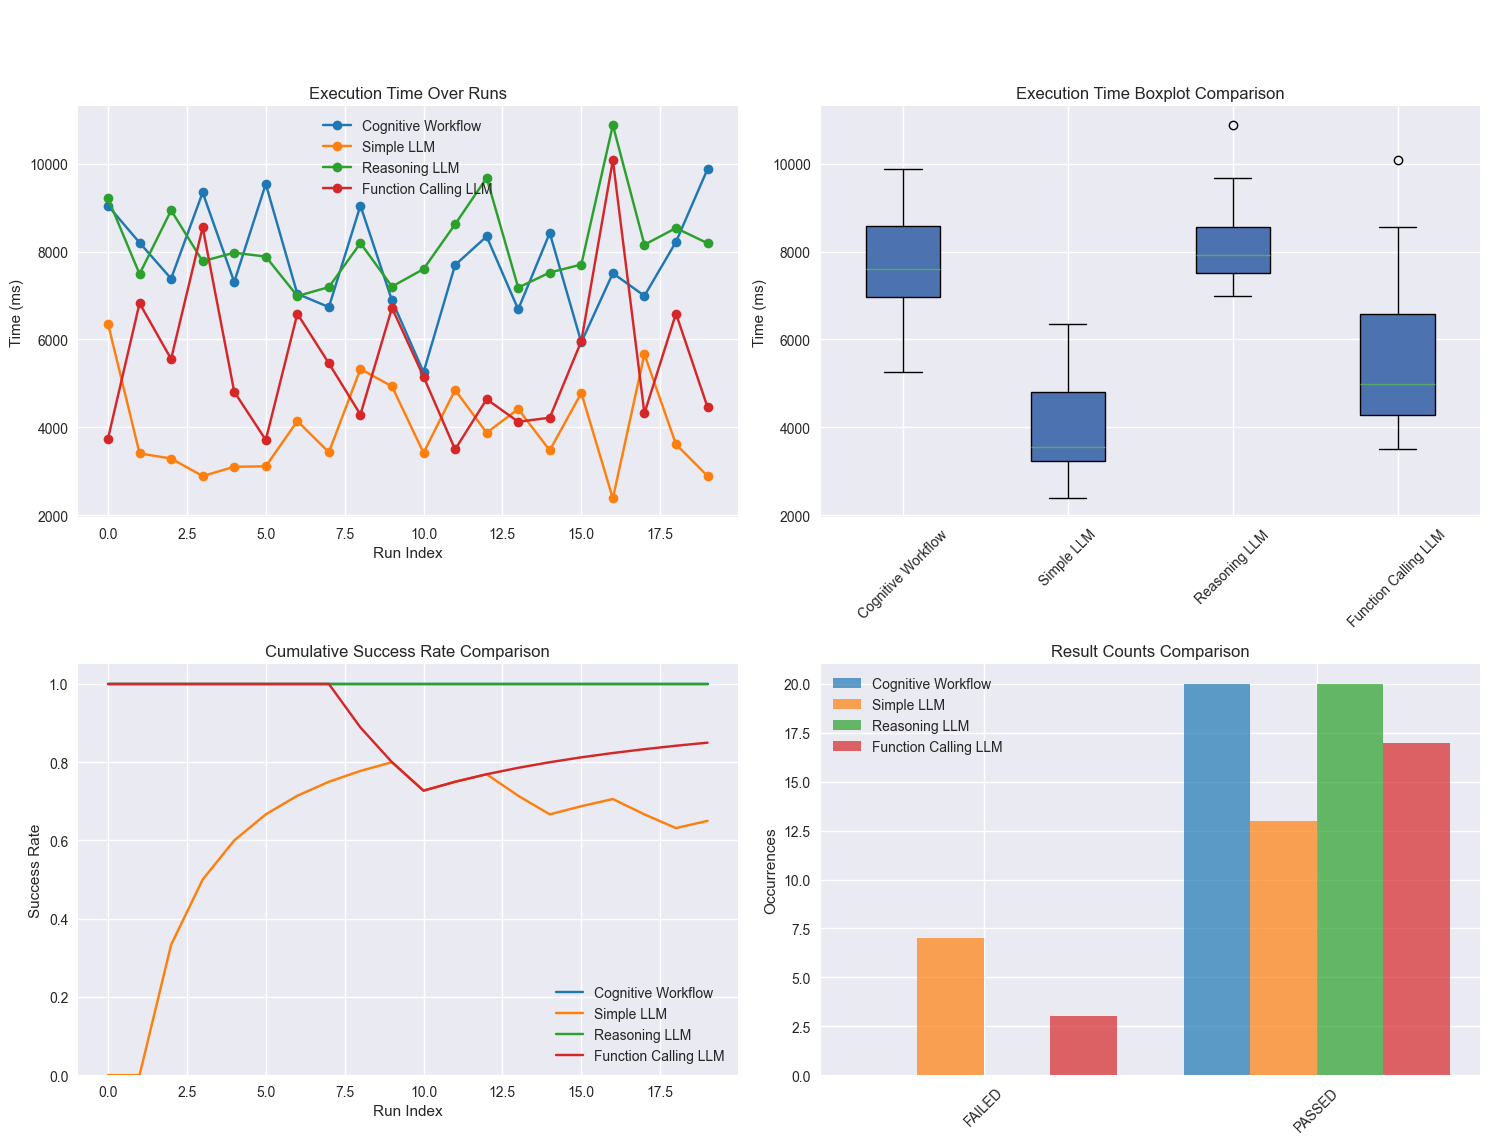
\includegraphics[width=1\textwidth]{Template_tesi/img/a4ne/1a.png}
\caption{Performance and reliability comparison of the four approaches under a 5G network routing scenario involving AI-enhanced signal processing.}
\label{fig:test1a}
\end{figure}


Another interesting and more challenging test case involved the same network, where the following configuration was requested:

\begin{promptboxcontent}
\small\textit{Configure a high-throughput network to process sensor fusion data from 500 Google Waymo autonomous vehicles for centralized AI training. Each vehicle streams 80 MB/s of LiDAR, camera, and radar data. A single processing node must ingest all incoming data streams, utilizing NVMe-over-Fabrics storage for training dataset ingestion and hardware-accelerated preprocessing before forwarding the data to downstream GPU training clusters.}
\end{promptboxcontent}
%\promptcaption{pr:network_config}{High‑Throughput Network Configuration Request}

This prompt is more demanding than the previous one. Rather than relying on basic feature matching from device manuals for hardware selection, it required mathematical reasoning to compute the total requested workload. Specifically, it was necessary to aggregate the input data rate as follows:

\begin{align*}
\text{Data rate per vehicle} &= 80~\text{MB/s} = 0.64~\text{Gb/s} \\
\text{Total for 500 vehicles} &= 500 \times 0.64 = 320~\text{Gb/s} \\
\text{With a requested 5\% margin} &= 320 \times 1.05 = \boxed{336~\text{Gb/s}}
\end{align*}

\noindent
This made the test unambiguous, since only one device, namely the NVIDIA BlueField-3 DPU, could meet the required throughput (up to 400 Gb/s).


\begin{figure}[h]
    \centering
    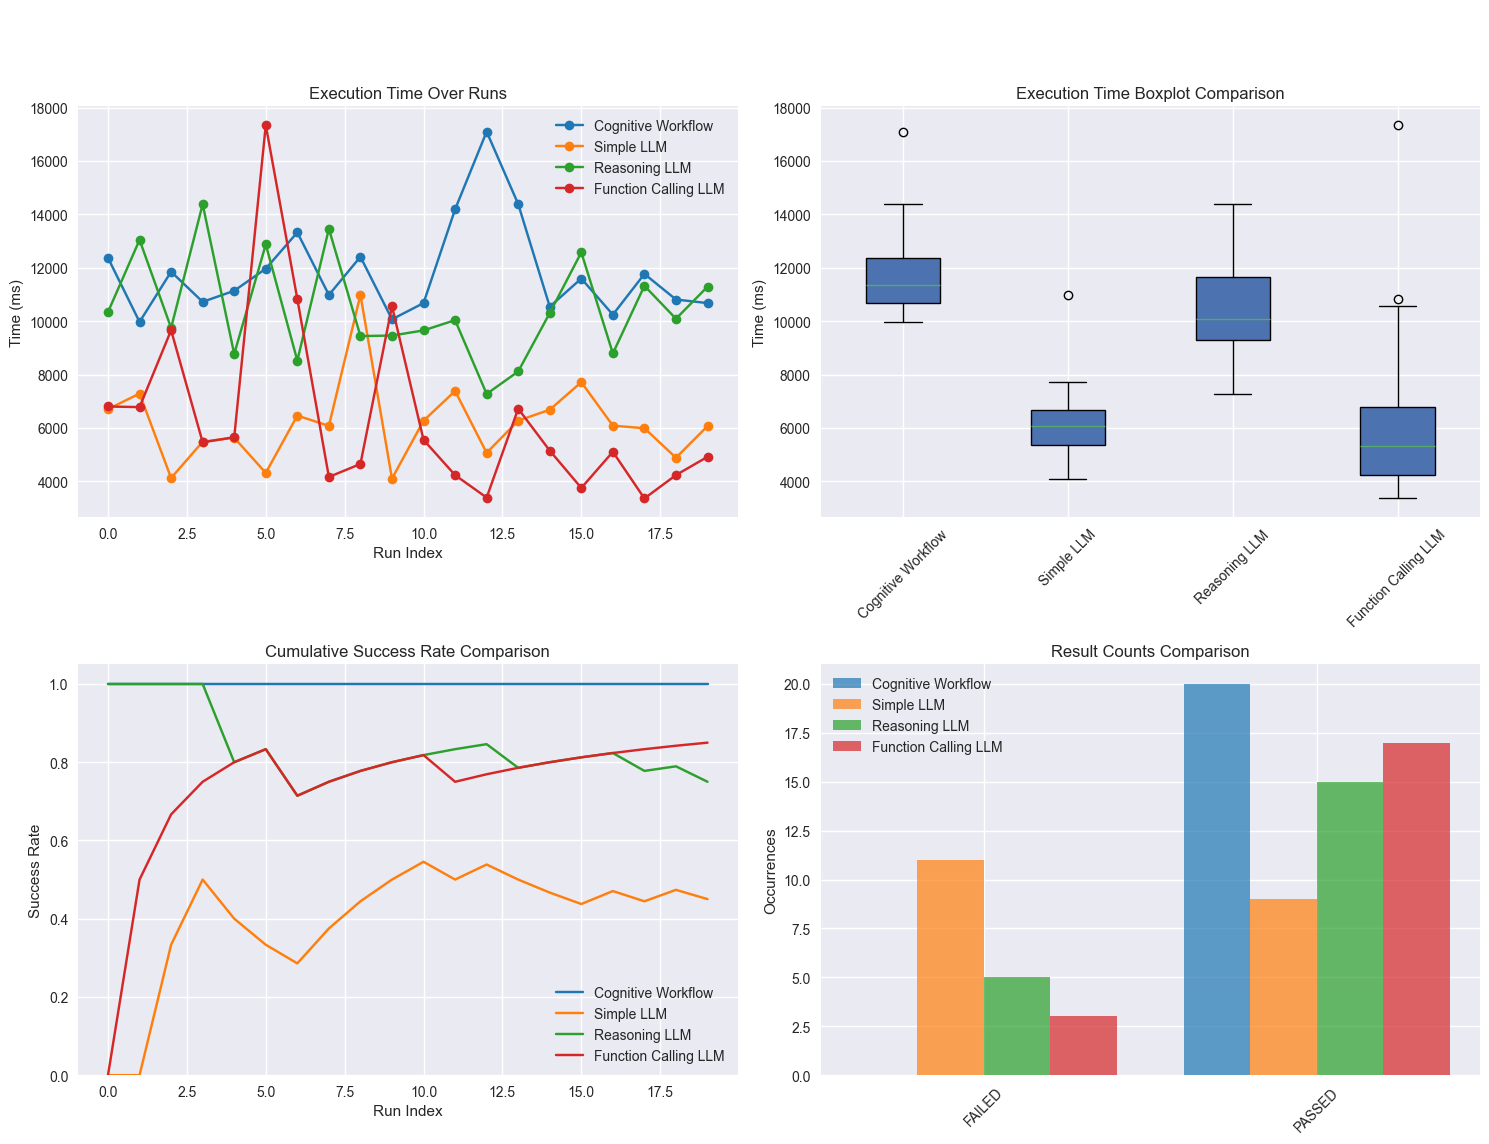
\includegraphics[width=1\textwidth]{Template_tesi/img/a4ne/1b.png}
    \caption{Performance and reliability comparison of the four approaches processing a complex network configuration scenario that requires aggregating multiple specifications and performing throughput calculations.}
    \label{fig:test1b} 
\end{figure}


In this scenario, the Cognitive Workflow once again achieved the highest accuracy, followed by the Function Calling agent. The Reasoning LLM, even without external tools, demonstrated a remarkable accuracy comparable to that of the Function Calling agent, though it was significantly slower. The Simple LLM, by contrast, had a success rate below 50\% (see Figure~\ref{fig:test1b}). 




\begin{figure}[h]
    \centering
    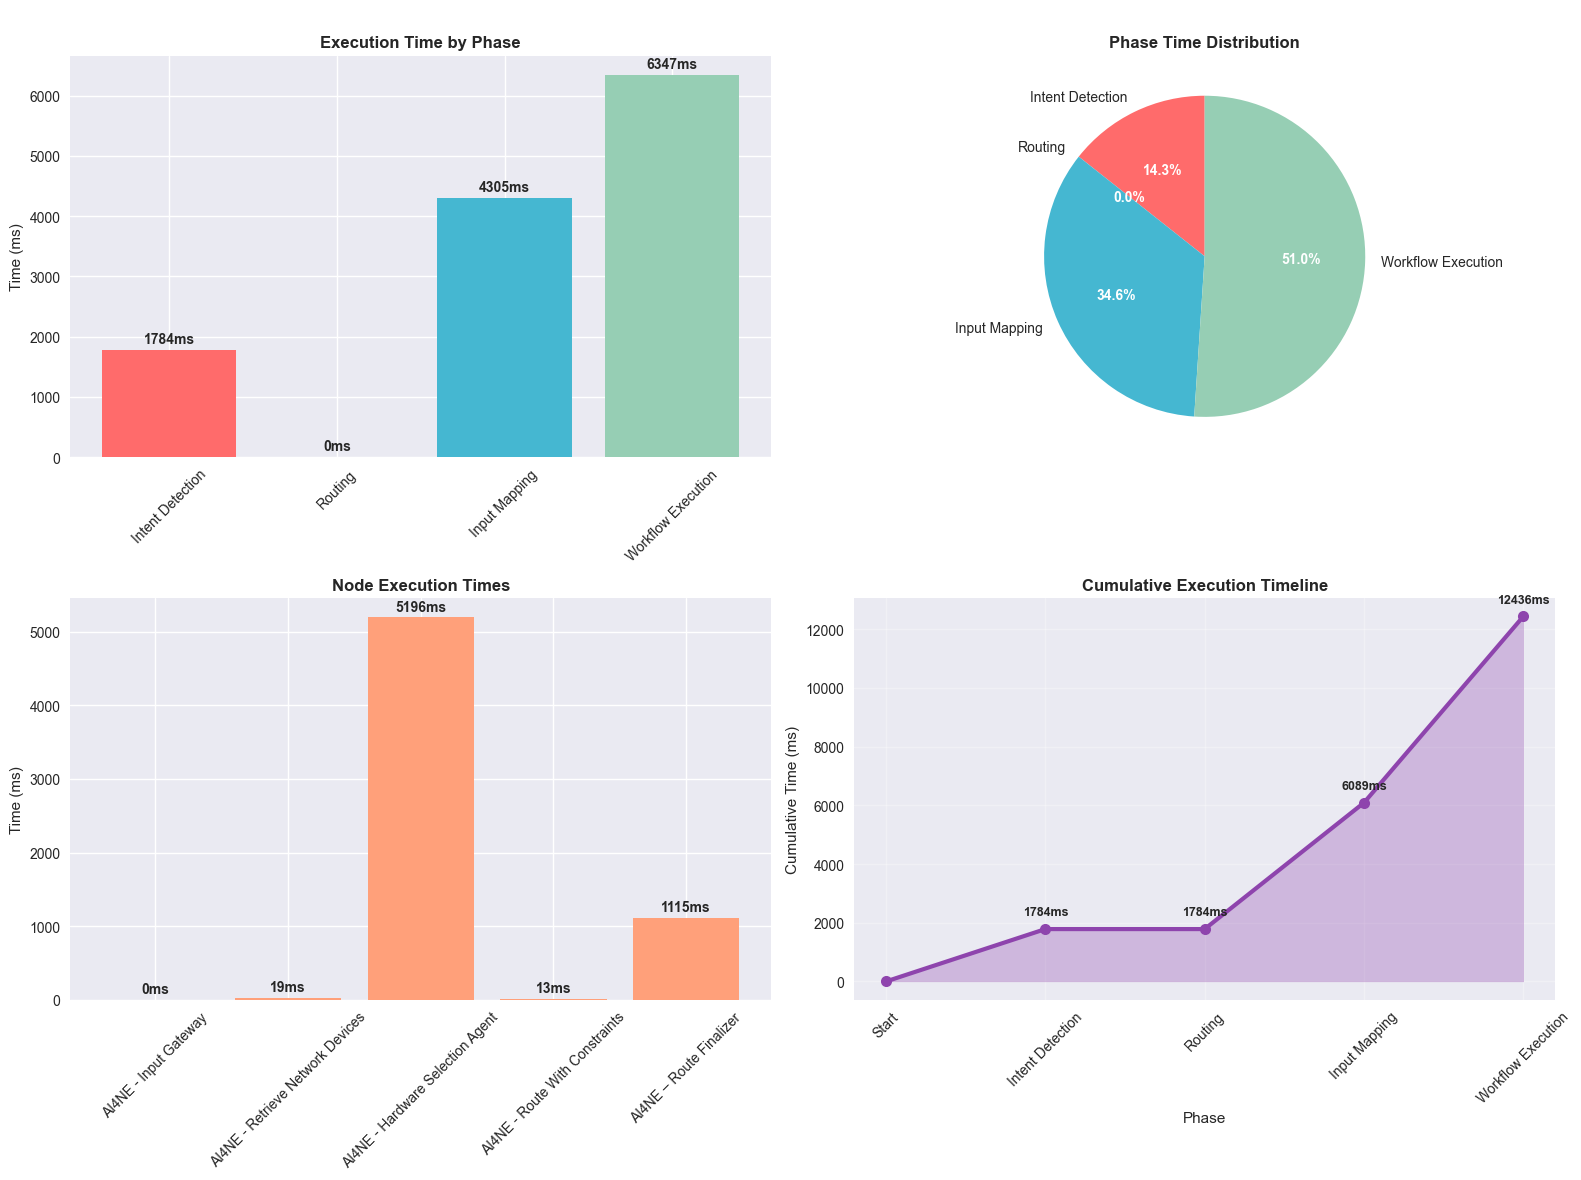
\includegraphics[width=1\textwidth]{Template_tesi/img/a4ne/observability.png}
    \caption{Execution time breakdown of a Cognitive Workflow, detailing phases including intent detection, input mapping, and subsequent processing steps.}
    \label{fig:time-breakdown} 
\end{figure}


Interestingly, execution times increased across all methods, particularly for the Cognitive Workflow. This was likely due to the mathematical reasoning required by the task, as well as, in the case of the Cognitive Workflow, the greater number of constraints expressed in the prompt—which extended both the intent detection and input mapping phases. The execution time breakdowns (Figure \ref{fig:time-breakdown}) support this observation: approximately 34.6\% of the total execution time was spent on input mapping, which took about 31.4\% more time in absolute terms compared to the first test scenario. Additionally, 14.3\% of the time was spent on intent detection, which introduced unnecessary overhead, given that only a single intent was involved. While these results highlight structural trade-offs between the two approaches, performance can still be improved through targeted optimizations, such as using smaller foundational models, applying prompt engineering techniques, and implementing caching strategies (see Section \ref{sec:next_steps}).




\subsection{Observations}
During the evaluation of the four approaches, we observed recurring patterns that offer critical insights:


\begin{itemize}[leftmargin=*, label=--]
\item \textbf{Tool Calling Inconsistency}: The function-calling setup exhibited inconsistencies in the execution of tools. Despite clear, step-by-step instructions and tool definitions, the system occasionally deviated from the expected flow—invoking tools out of order. For instance, it sometimes bypassed the routing tool entirely and attempted path selection autonomously, undermining the intended separation between reasoning and computation. In other cases, the same tools were invoked multiple times, resulting in unnecessary delays in execution.

\item \textbf{Self-Explanation Prompting}: All agents showed improved performance when prompted to justify their decisions, although this was accompanied by increased token usage. Notably, the single LLM variant, when not required to generate explicit explanations, frequently failed even on simple tasks. Instructing for motivations regarding the inclusion or exclusion of hardware devices also enhanced the accuracy of the Hardware Selector Node within the Cognitive Workflow.

\item \textbf{Chain-of-Thought Prompting}: Failures observed in the single-LLM setup were often not due to flawed logic or incorrect decision criteria but rather to incomplete or invalid output paths, even with self-explanation prompting. In several instances, paths were missing critical intermediate nodes, or the model incorrectly assumed the existence of edges not present in the actual topology. In other cases, the model failed to associate device identifiers with corresponding node identifiers properly. When the agent was guided to apply the Chain-of-Thought (CoT) prompting technique—breaking down the task into a series of reasoning steps, including hardware evaluation for each device, enumeration of connecting edges, and validation of the entire path—these topology-related errors were largely resolved. 

\item \textbf{Self-Contradiction}: Both the Simple LLM and the Function Calling agent occasionally produced outputs where the reasoning did not align with the final path selected. In several cases, the explanation referenced a combination of multiple selected devices, while the final result included only a single device. These inconsistencies suggest difficulties in maintaining coherent reasoning under complex, multi-constraint scenarios—especially when operating near token limits.


\end{itemize}

Additional implementation challenges for the Cognitive Workflow are discussed in Section \ref{sec:challenge}.



\subsection{Key Insights and Future Directions}


Several important insights and future considerations were revealed during the evaluation experiment:

\begin{itemize}[leftmargin=*, label=--]

  \item \textbf{Necessity of a more challenging evaluation framework}: The unexpectedly strong performance of the simple LLM in early tasks suggests that the test environment may be too simplistic to highlight the benefits of structured workflows effectively. A more demanding testbed should include:
    \begin{itemize}[leftmargin=2em, label=--]
      \item Network topologies that are too complex for an LLM to solve unaided, including multi-layered networks with compute and switch devices.
      \item Weighted graphs that accurately reflect real-world constraints, including latency and bandwidth.
      \item Greater device heterogeneity and volume to surpass the context limit of a single LLM.
    \end{itemize}

  \item \textbf{Improving Task Clarity}: A recurring challenge was formulating tasks that were both non-trivial and unambiguous. Although the tasks were designed to require multidimensional reasoning, we frequently encountered ambiguity in hardware selection, which compromised reproducibility. This was often due to under-specified constraints or vague prompt formulations. To address this, we propose formalizing natural language requests and qualitative attributes into structured, quantitative requirement vectors by estimating hardware requirements prior to hardware selection (e.g., minimum TFLOPS $\geq$ 15, maximum latency $\leq$ 20 ms, etc.). This approach may reduce the incidence of multiple equally plausible solutions.

\end{itemize}


\subsection{Conclusion}
This feasibility study demonstrates that LLMs when embedded within cognitive workflow architectures, can support complex decision-making processes—while also exposing significant limitations. Although the networking scenario served as a valuable practical demonstration, it is not intended as a comprehensive exploration of the domain. Nonetheless, these initial findings encourage deeper investigation  on LLM-based cognitive systems in both AI for Network Engineering (AI4NE) and Network Engineering for AI (NE4AI) contexts.

